\begin{landscape}
\begin{figure}[!]
    \centering
    \begin{subfigure}{1.4\textwidth}
    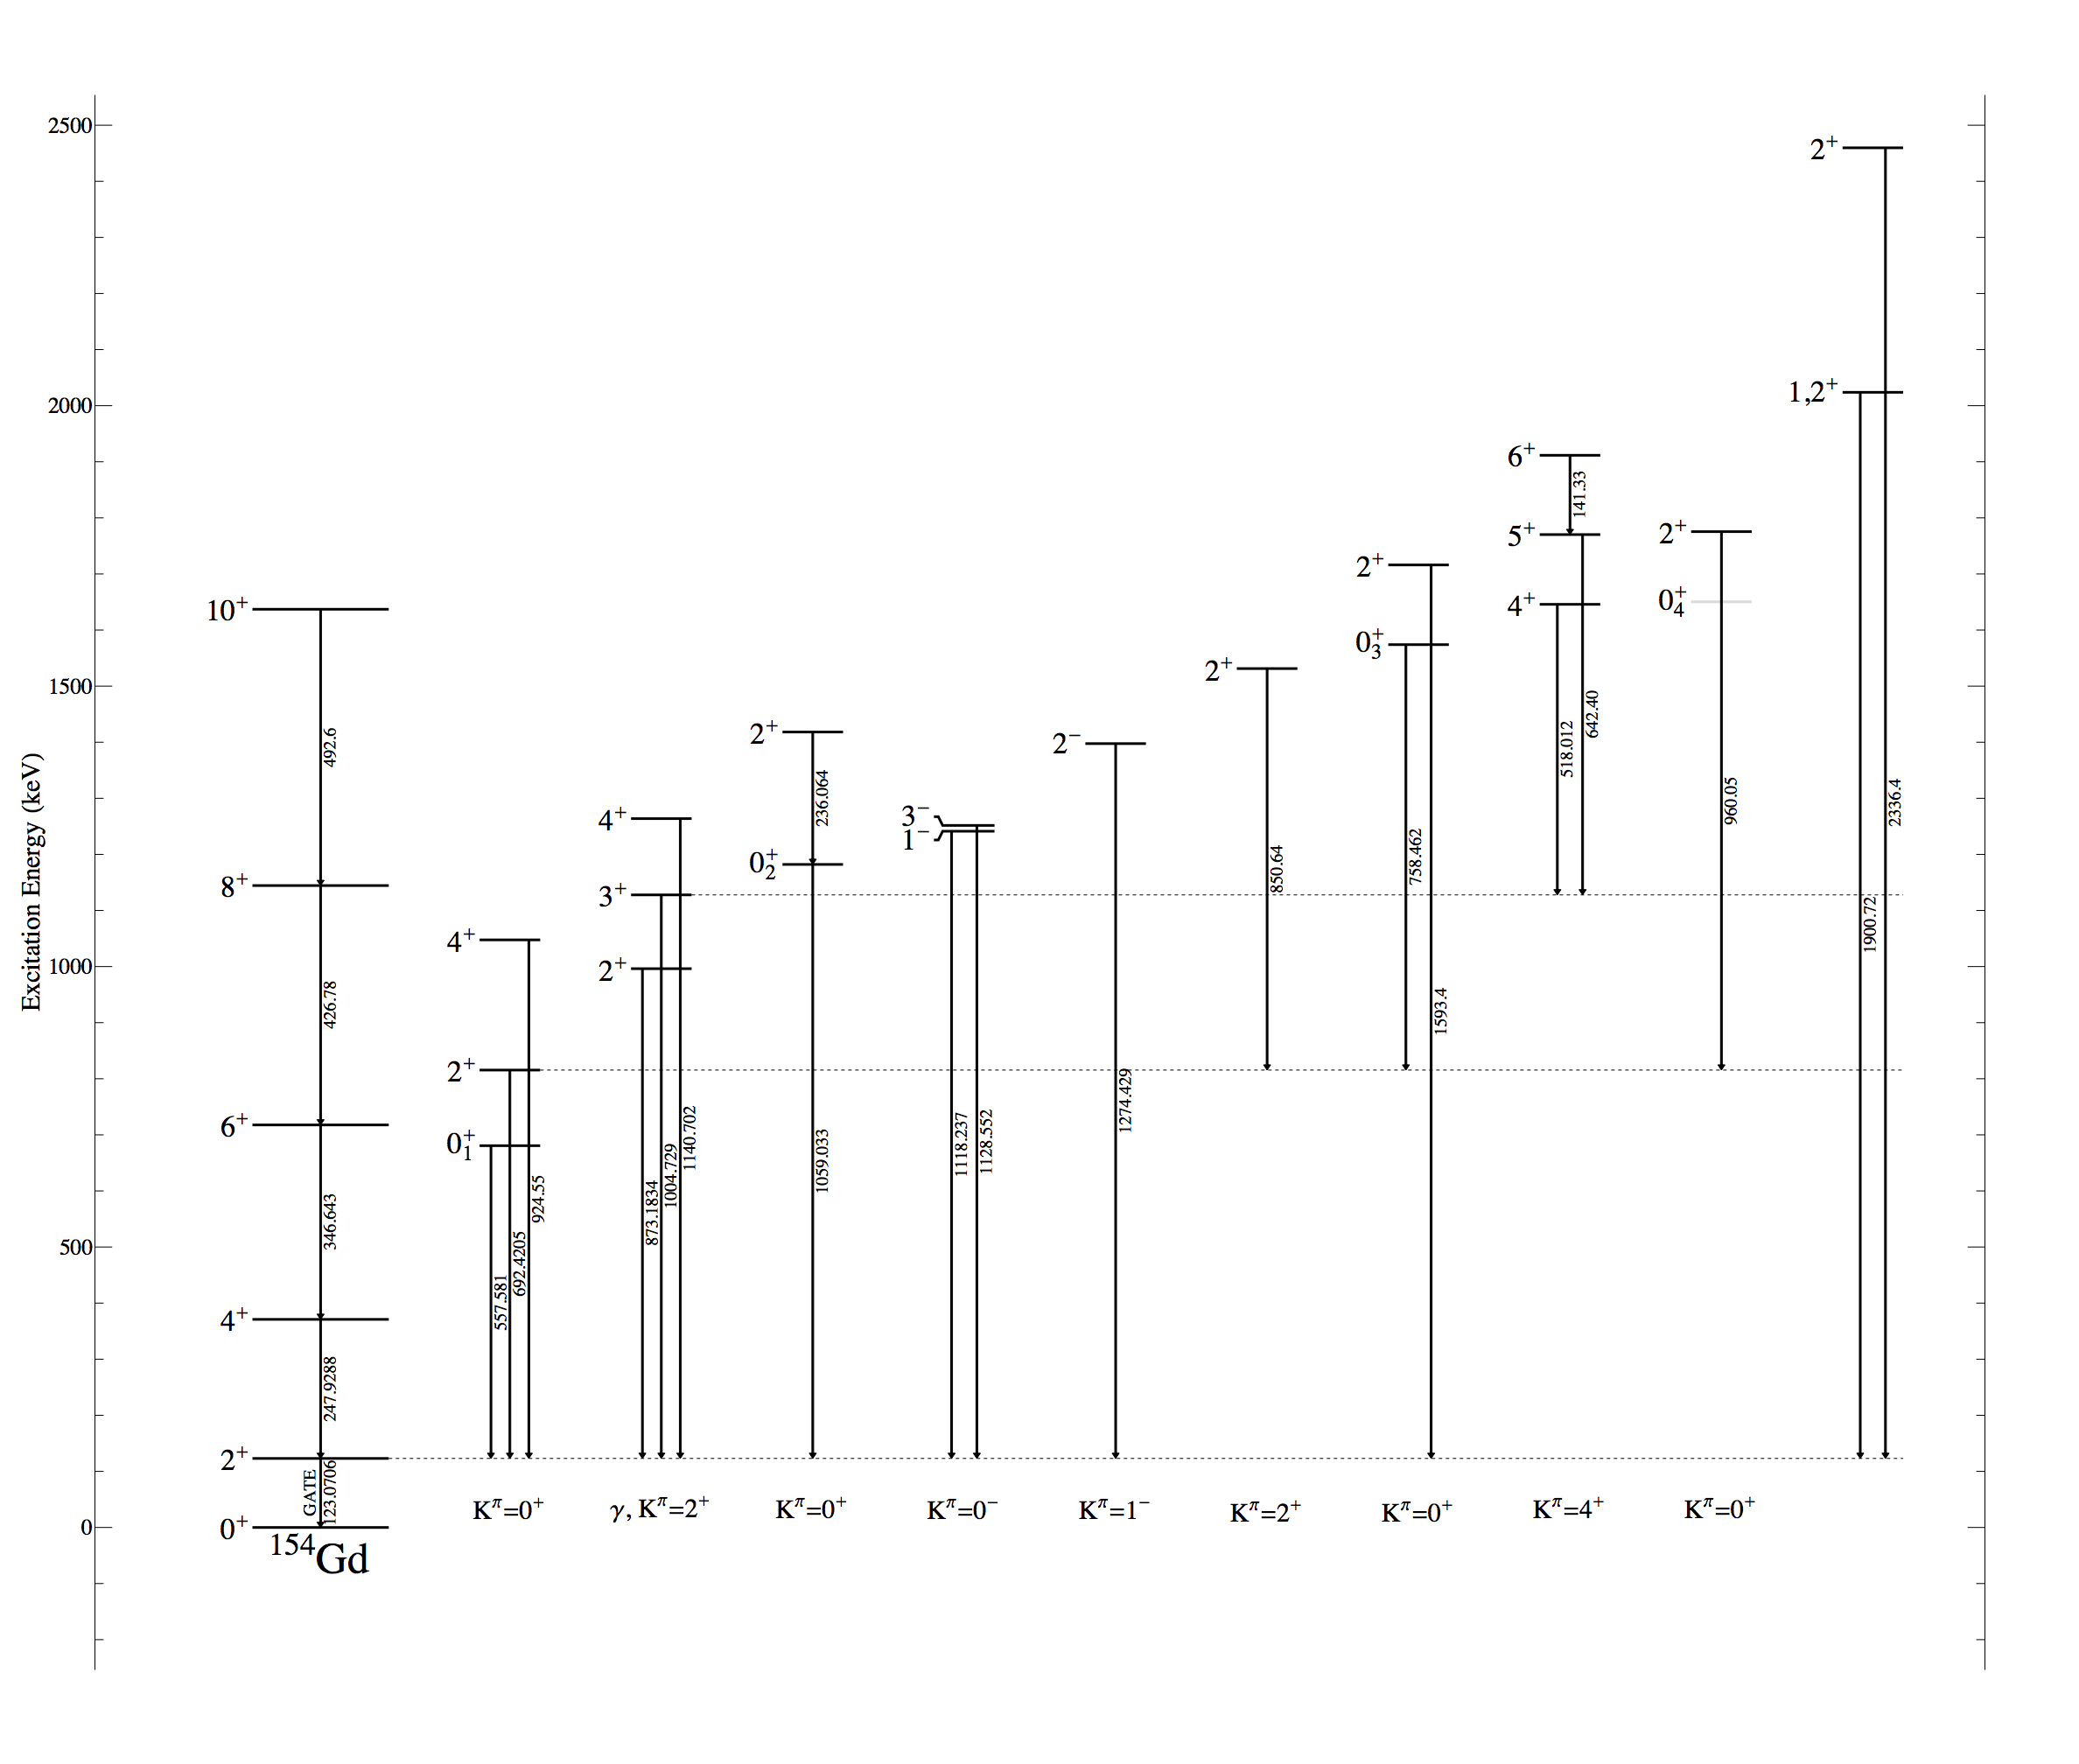
\includegraphics[scale=0.33]{154GdTablesAndFigs/154Gd_2to0.eps}
    \caption{\label{fig:154_2to0level}Level Scheme of $^{154}$Gd. The gamma ray of the $2^+\rightarrow0^+$ transition (123 keV) in the ground state was gated on. It was then compared with the gated spectrum from the gamma ray of the $4^+\rightarrow2^+$ transition (247 keV) in the ground state. Peaks only appearing in the first gate and not higher energy gates were assumed to go into the $2^+$ state, and assignments were made. Due to the low energy of the $2^+\rightarrow0^+$ transition, the efficiency was lower, and it is likely that transitions into the $2^+$ state were missed. The levels are organized by band. The lower levels of the band, unseen by gamma rays in this gate, are in gray.}
    \end{subfigure}
    \captionlistentry{Level scheme and spectrum of $^{154}$Gd based on the $2^+\rightarrow0^+$ transition.}
    \label{fig:154_2to0}
    \end{figure}
    \begin{figure}
    \ContinuedFloat
    \begin{subfigure}{1.4\textwidth}
    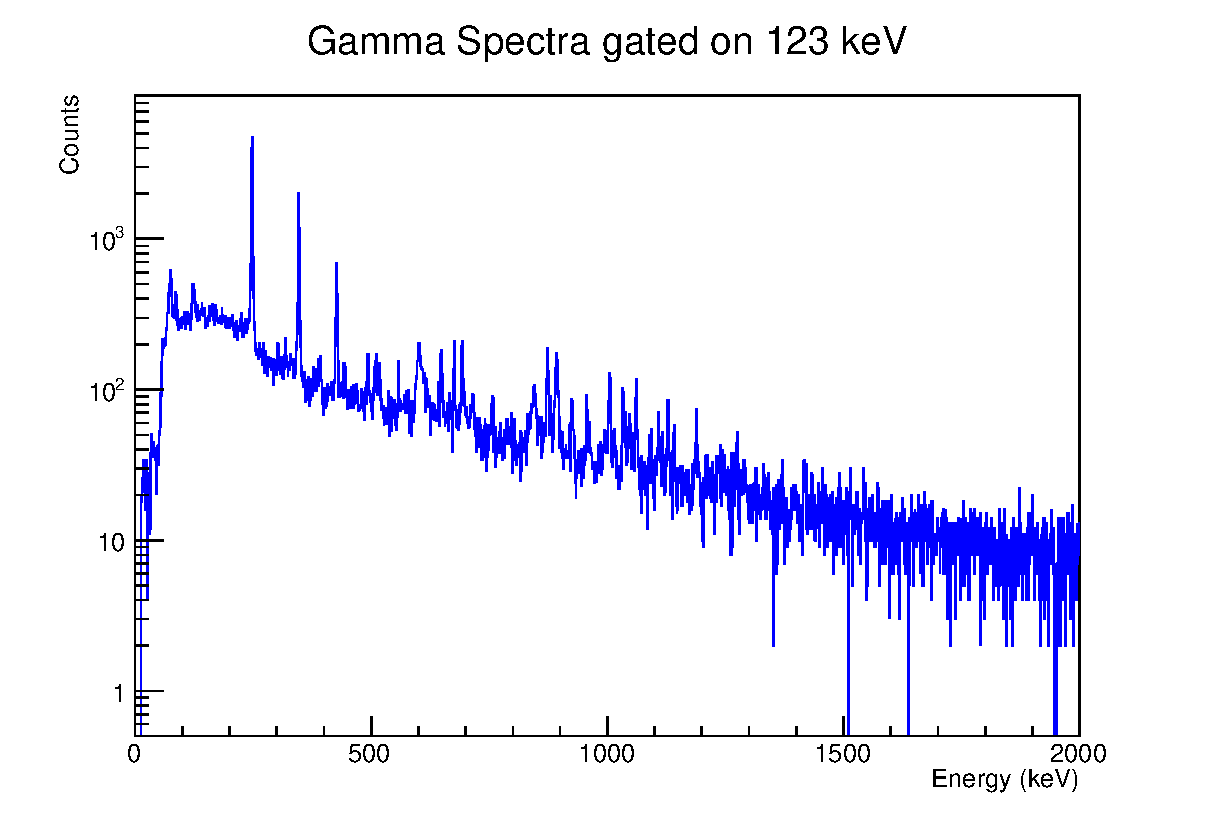
\includegraphics[]{154GdTablesAndFigs/123GateSpectrum.eps}
    \caption{Gamma spectrum gated on 123 keV, corresponding to the $2^+\rightarrow0^+$ transition.}
    \label{fig:154_2to0spec}
    \end{subfigure}
\end{figure}
\end{landscape}